\chapter{Obiekt symulowany - część projektowa}
Pierwszym etapem naszej pracy była analiza dostarczonego przez prowadzącego programu symulującego działanie obiektu. Był to obiekt dyskretny z opóźnieniem zależny od zmiennych procesu $U(k-11)$, $U(k-10)$, $Y(k-1)$, $Y(k-2)$.

Program do obsługi całego zadania symulacji został zaimplementowany w pliku \texttt{Projekt1.m}. Wykonywane są w nim wszystkie wymagane polecenia niezbędne do wykonania zadania, tj. sprawdzenie poprawności wartości w punkcie pracy $U_{\mathrm{pp}}$ i $Y_{\mathrm{pp}}$, wyznaczenie odpowiedzi skokowych procesu, wywołanie funkcji implementujących algorytmy PID i DMC, a także optymalizacja wskaźnika jakości regulacji $E$.

\section{Wyznaczenie odpowiedzi skokowych procesu}
Rozpoczynając od punktu pracy $U_{\mathrm{pp}}=\num{0,8}$ i $Y_{\mathrm{pp}}=2$ wyznaczaliśmy różne odpowiedzi skokowe dla kilku zmian sygnału sterującego. Wyniki symulacji przedstawione są na Rys.~\ref{os}. Jak widać, symulowany obiekt jest stabilny (charakterystyki po pewnym czasie ustalają się na stałym poziomie) oraz liniowy (charakterystyki statyczne $Y(U)$ leżą w przybliżeniu na linii prostej, co przedstawione jest na Rys.~\ref{char_stat}).

Na podstawie tej charakterystyki możemy obliczyć wzmocnienie statyczne procesu. Definiuje się je jako
\begin{equation}
K=\frac{\Delta Y}{\Delta U}
\end{equation}
Parametry $\Delta Y$ i $\Delta U$ są stałe dla dowolnie wybranych punktów na wykresie $Y(U)$, ponieważ charakterystyka jest liniowa. Należy więc wybrać dowolne punkty $(U_i, Y_i)$ i $(U_j, Y_j)$ i na ich podstawie obliczyć wzmocnienie statyczne $K$. Wynik:
\begin{equation}
K=1
\end{equation}

\begin{figure}
\label{os}
\centering
\caption{Odpowiedzi skokowe dla procesu symulowanego}
% This file was created by matlab2tikz.
%
\definecolor{mycolor1}{rgb}{1.00000,0.00000,1.00000}%
\definecolor{mycolor2}{rgb}{0.00000,1.00000,1.00000}%
%
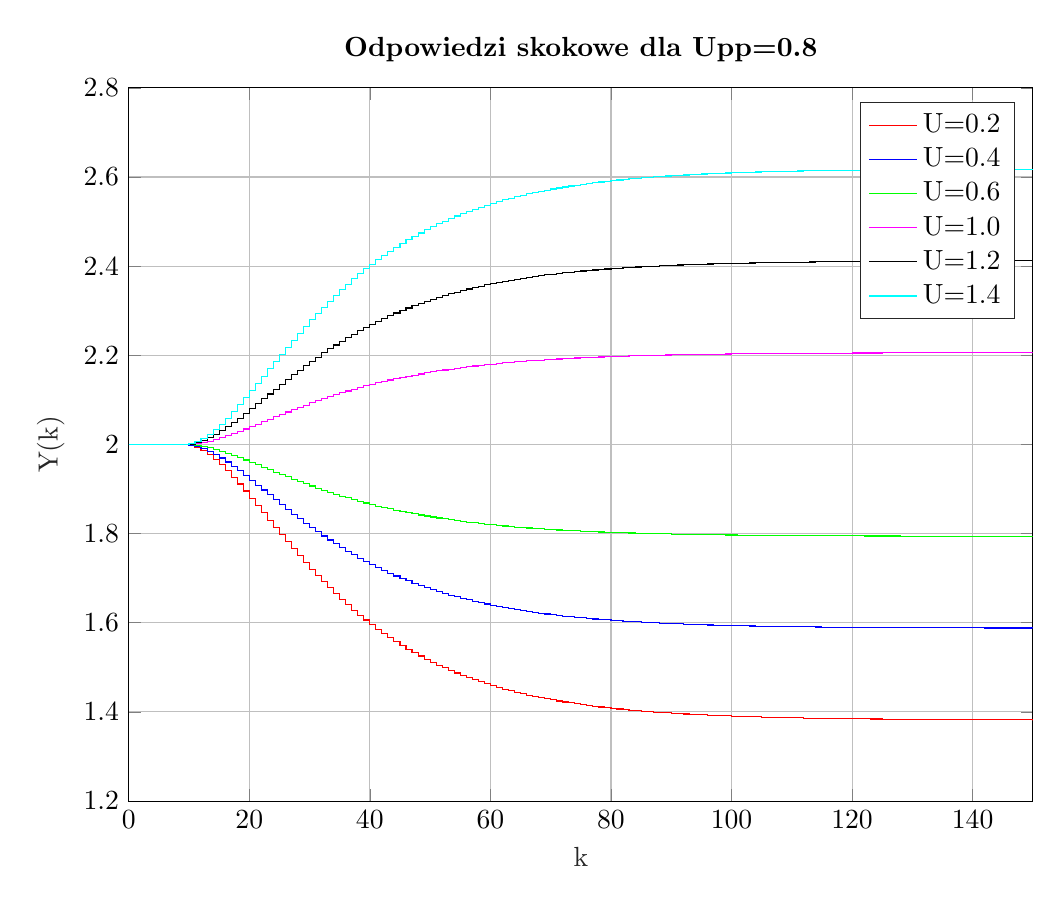
\begin{tikzpicture}

\begin{axis}[%
width=4.521in,
height=3.566in,
at={(0.758in,0.481in)},
scale only axis,
xmin=0,
xmax=150,
xlabel style={font=\color{white!15!black}},
xlabel={k},
ymin=1.2,
ymax=2.8,
ylabel style={font=\color{white!15!black}},
ylabel={Y(k)},
axis background/.style={fill=white},
title style={font=\bfseries},
title={Odpowiedzi skokowe dla Upp=0.8},
xmajorgrids,
ymajorgrids,
legend style={legend cell align=left, align=left, draw=white!15!black}
]
\addplot[const plot, color=red] table[row sep=crcr] {%
0	2\\
1	2\\
2	2\\
3	2\\
4	2\\
5	2\\
6	2\\
7	2\\
8	2\\
9	2\\
10	1.99836974\\
11	1.993804574792\\
12	1.98675077176943\\
13	1.9776031006434\\
14	1.96671022308248\\
15	1.95437954291634\\
16	1.94088156968435\\
17	1.92645384320798\\
18	1.9113044622537\\
19	1.89561525618372\\
20	1.87954463472339\\
21	1.86323014756816\\
22	1.84679078247401\\
23	1.83032902769341\\
24	1.81393272210415\\
25	1.79767671410647\\
26	1.78162434831043\\
27	1.76582879718065\\
28	1.75033425312912\\
29	1.73517699503257\\
30	1.72038634178294\\
31	1.70598550424369\\
32	1.69199234586852\\
33	1.67842006123113\\
34	1.66527778080386\\
35	1.65257110950162\\
36	1.64030260576434\\
37	1.62847220728182\\
38	1.61707760885926\\
39	1.60611459737593\\
40	1.59557734829637\\
41	1.58545868774896\\
42	1.57575032378499\\
43	1.56644305006941\\
44	1.55752692492794\\
45	1.54899142838022\\
46	1.5408255995233\\
47	1.53301815638995\\
48	1.52555760019054\\
49	1.51843230565225\\
50	1.51163059899408\\
51	1.50514082491827\\
52	1.49895140385573\\
53	1.49305088057565\\
54	1.48742796515313\\
55	1.4820715671855\\
56	1.47697082405375\\
57	1.47211512394192\\
58	1.46749412425114\\
59	1.46309776597717\\
60	1.45891628455902\\
61	1.45494021765133\\
62	1.45116041022364\\
63	1.44756801734544\\
64	1.44415450497611\\
65	1.44091164904313\\
66	1.43783153305977\\
67	1.43490654450505\\
68	1.43212937016277\\
69	1.42949299059359\\
70	1.42699067389351\\
71	1.42461596887342\\
72	1.42236269777852\\
73	1.42022494865097\\
74	1.41819706742667\\
75	1.41627364984496\\
76	1.41444953323988\\
77	1.41271978827207\\
78	1.4110797106526\\
79	1.40952481290224\\
80	1.40805081618348\\
81	1.40665364223685\\
82	1.40532940544786\\
83	1.4040744050667\\
84	1.4028851175984\\
85	1.40175818937833\\
86	1.40069042934424\\
87	1.39967880201383\\
88	1.39872042067429\\
89	1.39781254078826\\
90	1.39695255361896\\
91	1.39613798007566\\
92	1.39536646477943\\
93	1.3946357703478\\
94	1.39394377189641\\
95	1.39328845175437\\
96	1.39266789438998\\
97	1.39208028154234\\
98	1.39152388755441\\
99	1.39099707490234\\
100	1.39049828991594\\
101	1.39002605868451\\
102	1.38957898314264\\
103	1.38915573732998\\
104	1.38875506381921\\
105	1.38837577030638\\
106	1.38801672635763\\
107	1.38767686030665\\
108	1.38735515629701\\
109	1.38705065146363\\
110	1.38676243324802\\
111	1.38648963684166\\
112	1.38623144275223\\
113	1.38598707448758\\
114	1.38575579635226\\
115	1.38553691135188\\
116	1.38532975920029\\
117	1.38513371442538\\
118	1.38494818456859\\
119	1.38477260847429\\
120	1.38460645466458\\
121	1.38444921979572\\
122	1.38430042719231\\
123	1.38415962545559\\
124	1.38402638714221\\
125	1.38390030751035\\
126	1.38378100332965\\
127	1.38366811175211\\
128	1.38356128924083\\
129	1.38346021055382\\
130	1.38336456778021\\
131	1.38327406942618\\
132	1.38318843954819\\
133	1.38310741693113\\
134	1.38303075430927\\
135	1.38295821762756\\
136	1.38288958534161\\
137	1.38282464775412\\
138	1.38276320638603\\
139	1.3827050733806\\
140	1.38265007093876\\
141	1.38259803078406\\
142	1.38254879365582\\
143	1.38250220882889\\
144	1.38245813365874\\
145	1.38241643315059\\
146	1.38237697955126\\
147	1.38233965196255\\
148	1.38230433597519\\
149	1.38227092332205\\
150	1.38223931154985\\
};
\addlegendentry{U=0.2}

\addplot[const plot, color=blue] table[row sep=crcr] {%
0	2\\
1	2\\
2	2\\
3	2\\
4	2\\
5	2\\
6	2\\
7	2\\
8	2\\
9	2\\
10	1.99891316\\
11	1.995869716528\\
12	1.99116718117962\\
13	1.98506873376227\\
14	1.97780681538832\\
15	1.96958636194423\\
16	1.9605877131229\\
17	1.95096922880532\\
18	1.94086964150247\\
19	1.93041017078914\\
20	1.91969642314893\\
21	1.90882009837877\\
22	1.89786052164934\\
23	1.88688601846227\\
24	1.87595514806944\\
25	1.86511780940432\\
26	1.85441623220696\\
27	1.8438858647871\\
28	1.83355616875275\\
29	1.82345133002171\\
30	1.81359089452196\\
31	1.80399033616246\\
32	1.79466156391235\\
33	1.78561337415408\\
34	1.77685185386924\\
35	1.76838073966775\\
36	1.76020173717623\\
37	1.75231480485455\\
38	1.74471840590618\\
39	1.73740973158395\\
40	1.73038489886425\\
41	1.72363912516598\\
42	1.71716688252333\\
43	1.71096203337961\\
44	1.70501794995197\\
45	1.69932761892015\\
46	1.69388373301554\\
47	1.68867877092664\\
48	1.6837050667937\\
49	1.67895487043484\\
50	1.67442039932939\\
51	1.67009388327885\\
52	1.66596760257049\\
53	1.66203392038377\\
54	1.65828531010209\\
55	1.65471437812367\\
56	1.6513138827025\\
57	1.64807674929462\\
58	1.6449960828341\\
59	1.64206517731812\\
60	1.63927752303935\\
61	1.63662681176756\\
62	1.6341069401491\\
63	1.63171201156363\\
64	1.62943633665074\\
65	1.62727443269542\\
66	1.62522102203985\\
67	1.62327102967004\\
68	1.62141958010851\\
69	1.61966199372906\\
70	1.61799378259567\\
71	1.61641064591562\\
72	1.61490846518568\\
73	1.61348329910065\\
74	1.61213137828445\\
75	1.61084909989664\\
76	1.60963302215992\\
77	1.60847985884805\\
78	1.6073864737684\\
79	1.60634987526816\\
80	1.60536721078899\\
81	1.60443576149123\\
82	1.60355293696524\\
83	1.60271627004447\\
84	1.60192341173227\\
85	1.60117212625222\\
86	1.60046028622949\\
87	1.59978586800922\\
88	1.59914694711619\\
89	1.59854169385884\\
90	1.5979683690793\\
91	1.59742532005044\\
92	1.59691097651962\\
93	1.59642384689853\\
94	1.5959625145976\\
95	1.59552563450291\\
96	1.59511192959332\\
97	1.59472018769489\\
98	1.5943492583696\\
99	1.59399804993489\\
100	1.59366552661062\\
101	1.59335070578967\\
102	1.59305265542842\\
103	1.59277049155331\\
104	1.59250337587947\\
105	1.59225051353758\\
106	1.59201115090508\\
107	1.59178457353776\\
108	1.591570104198\\
109	1.59136710097574\\
110	1.59117495549867\\
111	1.59099309122776\\
112	1.59082096183481\\
113	1.59065804965838\\
114	1.59050386423484\\
115	1.59035794090124\\
116	1.59021983946686\\
117	1.59008914295025\\
118	1.58996545637906\\
119	1.58984840564952\\
120	1.58973763644305\\
121	1.58963281319714\\
122	1.5895336181282\\
123	1.58943975030372\\
124	1.58935092476147\\
125	1.58926687167356\\
126	1.5891873355531\\
127	1.5891120745014\\
128	1.58904085949388\\
129	1.58897347370254\\
130	1.58890971185347\\
131	1.58884937961745\\
132	1.58879229303212\\
133	1.58873827795408\\
134	1.58868716953951\\
135	1.5886388117517\\
136	1.5885930568944\\
137	1.58854976516941\\
138	1.58850880425735\\
139	1.5884700489204\\
140	1.58843338062584\\
141	1.58839868718937\\
142	1.58836586243721\\
143	1.58833480588592\\
144	1.58830542243915\\
145	1.58827762210039\\
146	1.58825131970084\\
147	1.5882264346417\\
148	1.58820289065012\\
149	1.58818061554803\\
150	1.58815954103323\\
};
\addlegendentry{U=0.4}

\addplot[const plot, color=green] table[row sep=crcr] {%
0	2\\
1	2\\
2	2\\
3	2\\
4	2\\
5	2\\
6	2\\
7	2\\
8	2\\
9	2\\
10	1.99945658\\
11	1.997934858264\\
12	1.99558359058981\\
13	1.99253436688113\\
14	1.98890340769416\\
15	1.98479318097211\\
16	1.98029385656145\\
17	1.97548461440266\\
18	1.97043482075123\\
19	1.96520508539457\\
20	1.95984821157446\\
21	1.95441004918939\\
22	1.94893026082467\\
23	1.94344300923114\\
24	1.93797757403472\\
25	1.93255890470216\\
26	1.92720811610348\\
27	1.92194293239355\\
28	1.91677808437637\\
29	1.91172566501086\\
30	1.90679544726098\\
31	1.90199516808123\\
32	1.89733078195617\\
33	1.89280668707704\\
34	1.88842592693462\\
35	1.88419036983387\\
36	1.88010086858811\\
37	1.87615740242727\\
38	1.87235920295309\\
39	1.86870486579198\\
40	1.86519244943212\\
41	1.86181956258299\\
42	1.85858344126167\\
43	1.85548101668981\\
44	1.85250897497598\\
45	1.84966380946008\\
46	1.84694186650777\\
47	1.84433938546332\\
48	1.84185253339685\\
49	1.83947743521742\\
50	1.8372101996647\\
51	1.83504694163943\\
52	1.83298380128525\\
53	1.83101696019189\\
54	1.82914265505105\\
55	1.82735718906184\\
56	1.82565694135125\\
57	1.82403837464731\\
58	1.82249804141705\\
59	1.82103258865906\\
60	1.81963876151968\\
61	1.81831340588378\\
62	1.81705347007455\\
63	1.81585600578182\\
64	1.81471816832537\\
65	1.81363721634771\\
66	1.81261051101993\\
67	1.81163551483502\\
68	1.81070979005426\\
69	1.80983099686453\\
70	1.80899689129784\\
71	1.80820532295781\\
72	1.80745423259284\\
73	1.80674164955033\\
74	1.80606568914223\\
75	1.80542454994832\\
76	1.80481651107996\\
77	1.80423992942403\\
78	1.8036932368842\\
79	1.80317493763408\\
80	1.8026836053945\\
81	1.80221788074562\\
82	1.80177646848262\\
83	1.80135813502224\\
84	1.80096170586614\\
85	1.80058606312611\\
86	1.80023014311475\\
87	1.79989293400461\\
88	1.7995734735581\\
89	1.79927084692942\\
90	1.79898418453966\\
91	1.79871266002522\\
92	1.79845548825981\\
93	1.79821192344927\\
94	1.79798125729881\\
95	1.79776281725146\\
96	1.79755596479666\\
97	1.79736009384745\\
98	1.7971746291848\\
99	1.79699902496745\\
100	1.79683276330531\\
101	1.79667535289484\\
102	1.79652632771421\\
103	1.79638524577666\\
104	1.79625168793974\\
105	1.79612525676879\\
106	1.79600557545254\\
107	1.79589228676888\\
108	1.795785052099\\
109	1.79568355048787\\
110	1.79558747774934\\
111	1.79549654561388\\
112	1.79541048091741\\
113	1.79532902482919\\
114	1.79525193211742\\
115	1.79517897045062\\
116	1.79510991973343\\
117	1.79504457147512\\
118	1.79498272818953\\
119	1.79492420282476\\
120	1.79486881822152\\
121	1.79481640659857\\
122	1.7947668090641\\
123	1.79471987515186\\
124	1.79467546238074\\
125	1.79463343583678\\
126	1.79459366777655\\
127	1.7945560372507\\
128	1.79452042974694\\
129	1.79448673685127\\
130	1.79445485592674\\
131	1.79442468980873\\
132	1.79439614651606\\
133	1.79436913897704\\
134	1.79434358476976\\
135	1.79431940587585\\
136	1.7942965284472\\
137	1.79427488258471\\
138	1.79425440212868\\
139	1.7942350244602\\
140	1.79421669031292\\
141	1.79419934359469\\
142	1.79418293121861\\
143	1.79416740294296\\
144	1.79415271121958\\
145	1.7941388110502\\
146	1.79412565985042\\
147	1.79411321732085\\
148	1.79410144532506\\
149	1.79409030777402\\
150	1.79407977051661\\
};
\addlegendentry{U=0.6}

\addplot[const plot, color=mycolor1] table[row sep=crcr] {%
0	2\\
1	2\\
2	2\\
3	2\\
4	2\\
5	2\\
6	2\\
7	2\\
8	2\\
9	2\\
10	2.00054342\\
11	2.002065141736\\
12	2.00441640941019\\
13	2.00746563311887\\
14	2.01109659230584\\
15	2.01520681902789\\
16	2.01970614343855\\
17	2.02451538559734\\
18	2.02956517924877\\
19	2.03479491460543\\
20	2.04015178842554\\
21	2.04558995081062\\
22	2.05106973917533\\
23	2.05655699076887\\
24	2.06202242596528\\
25	2.06744109529784\\
26	2.07279188389652\\
27	2.07805706760645\\
28	2.08322191562363\\
29	2.08827433498915\\
30	2.09320455273902\\
31	2.09800483191877\\
32	2.10266921804382\\
33	2.10719331292296\\
34	2.11157407306538\\
35	2.11580963016613\\
36	2.11989913141189\\
37	2.12384259757272\\
38	2.12764079704691\\
39	2.13129513420802\\
40	2.13480755056787\\
41	2.13818043741701\\
42	2.14141655873833\\
43	2.14451898331019\\
44	2.14749102502402\\
45	2.15033619053992\\
46	2.15305813349223\\
47	2.15566061453668\\
48	2.15814746660315\\
49	2.16052256478258\\
50	2.1627898003353\\
51	2.16495305836057\\
52	2.16701619871475\\
53	2.16898303980811\\
54	2.17085734494895\\
55	2.17264281093816\\
56	2.17434305864875\\
57	2.17596162535269\\
58	2.17750195858295\\
59	2.17896741134094\\
60	2.18036123848032\\
61	2.18168659411622\\
62	2.18294652992545\\
63	2.18414399421819\\
64	2.18528183167463\\
65	2.18636278365229\\
66	2.18738948898008\\
67	2.18836448516498\\
68	2.18929020994574\\
69	2.19016900313547\\
70	2.19100310870216\\
71	2.19179467704219\\
72	2.19254576740716\\
73	2.19325835044968\\
74	2.19393431085778\\
75	2.19457545005168\\
76	2.19518348892004\\
77	2.19576007057598\\
78	2.1963067631158\\
79	2.19682506236592\\
80	2.19731639460551\\
81	2.19778211925439\\
82	2.19822353151738\\
83	2.19864186497777\\
84	2.19903829413387\\
85	2.19941393687389\\
86	2.19976985688525\\
87	2.20010706599539\\
88	2.2004265264419\\
89	2.20072915307058\\
90	2.20101581546035\\
91	2.20128733997478\\
92	2.20154451174019\\
93	2.20178807655074\\
94	2.2020187427012\\
95	2.20223718274855\\
96	2.20244403520334\\
97	2.20263990615256\\
98	2.2028253708152\\
99	2.20300097503256\\
100	2.20316723669469\\
101	2.20332464710517\\
102	2.20347367228579\\
103	2.20361475422334\\
104	2.20374831206026\\
105	2.20387474323121\\
106	2.20399442454746\\
107	2.20410771323112\\
108	2.204214947901\\
109	2.20431644951213\\
110	2.20441252225066\\
111	2.20450345438612\\
112	2.20458951908259\\
113	2.20467097517081\\
114	2.20474806788258\\
115	2.20482102954937\\
116	2.20489008026657\\
117	2.20495542852487\\
118	2.20501727181047\\
119	2.20507579717524\\
120	2.20513118177847\\
121	2.20518359340143\\
122	2.20523319093589\\
123	2.20528012484814\\
124	2.20532453761926\\
125	2.20536656416321\\
126	2.20540633222345\\
127	2.20544396274929\\
128	2.20547957025305\\
129	2.20551326314872\\
130	2.20554514407326\\
131	2.20557531019127\\
132	2.20560385348394\\
133	2.20563086102295\\
134	2.20565641523024\\
135	2.20568059412414\\
136	2.20570347155279\\
137	2.20572511741529\\
138	2.20574559787132\\
139	2.2057649755398\\
140	2.20578330968708\\
141	2.20580065640531\\
142	2.20581706878139\\
143	2.20583259705704\\
144	2.20584728878042\\
145	2.2058611889498\\
146	2.20587434014958\\
147	2.20588678267915\\
148	2.20589855467494\\
149	2.20590969222599\\
150	2.20592022948339\\
};
\addlegendentry{U=1.0}

\addplot[const plot, color=black] table[row sep=crcr] {%
0	2\\
1	2\\
2	2\\
3	2\\
4	2\\
5	2\\
6	2\\
7	2\\
8	2\\
9	2\\
10	2.00108684\\
11	2.004130283472\\
12	2.00883281882038\\
13	2.01493126623773\\
14	2.02219318461168\\
15	2.03041363805577\\
16	2.0394122868771\\
17	2.04903077119468\\
18	2.05913035849753\\
19	2.06958982921086\\
20	2.08030357685107\\
21	2.09117990162123\\
22	2.10213947835066\\
23	2.11311398153773\\
24	2.12404485193056\\
25	2.13488219059568\\
26	2.14558376779304\\
27	2.1561141352129\\
28	2.16644383124725\\
29	2.17654866997829\\
30	2.18640910547804\\
31	2.19600966383754\\
32	2.20533843608765\\
33	2.21438662584592\\
34	2.22314814613076\\
35	2.23161926033225\\
36	2.23979826282377\\
37	2.24768519514545\\
38	2.25528159409382\\
39	2.26259026841605\\
40	2.26961510113575\\
41	2.27636087483402\\
42	2.28283311747667\\
43	2.28903796662039\\
44	2.29498205004803\\
45	2.30067238107984\\
46	2.30611626698446\\
47	2.31132122907336\\
48	2.3162949332063\\
49	2.32104512956516\\
50	2.32557960067061\\
51	2.32990611672115\\
52	2.33403239742951\\
53	2.33796607961623\\
54	2.34171468989791\\
55	2.34528562187633\\
56	2.3486861172975\\
57	2.35192325070538\\
58	2.3550039171659\\
59	2.35793482268188\\
60	2.36072247696065\\
61	2.36337318823244\\
62	2.3658930598509\\
63	2.36828798843637\\
64	2.37056366334926\\
65	2.37272556730458\\
66	2.37477897796015\\
67	2.37672897032996\\
68	2.37858041989148\\
69	2.38033800627093\\
70	2.38200621740432\\
71	2.38358935408438\\
72	2.38509153481431\\
73	2.38651670089935\\
74	2.38786862171555\\
75	2.38915090010335\\
76	2.39036697784007\\
77	2.39152014115195\\
78	2.39261352623159\\
79	2.39365012473183\\
80	2.394632789211\\
81	2.39556423850876\\
82	2.39644706303475\\
83	2.39728372995553\\
84	2.39807658826773\\
85	2.39882787374777\\
86	2.3995397137705\\
87	2.40021413199077\\
88	2.4008530528838\\
89	2.40145830614115\\
90	2.40203163092069\\
91	2.40257467994955\\
92	2.40308902348038\\
93	2.40357615310146\\
94	2.40403748540239\\
95	2.40447436549708\\
96	2.40488807040667\\
97	2.4052798123051\\
98	2.40565074163039\\
99	2.4060019500651\\
100	2.40633447338937\\
101	2.40664929421033\\
102	2.40694734457157\\
103	2.40722950844668\\
104	2.40749662412053\\
105	2.40774948646242\\
106	2.40798884909492\\
107	2.40821542646223\\
108	2.408429895802\\
109	2.40863289902425\\
110	2.40882504450133\\
111	2.40900690877224\\
112	2.40917903816519\\
113	2.40934195034162\\
114	2.40949613576516\\
115	2.40964205909876\\
116	2.40978016053314\\
117	2.40991085704975\\
118	2.41003454362094\\
119	2.41015159435048\\
120	2.41026236355695\\
121	2.41036718680286\\
122	2.4104663818718\\
123	2.41056024969628\\
124	2.41064907523853\\
125	2.41073312832644\\
126	2.4108126644469\\
127	2.4108879254986\\
128	2.41095914050612\\
129	2.41102652629746\\
130	2.41109028814653\\
131	2.41115062038255\\
132	2.41120770696788\\
133	2.41126172204591\\
134	2.41131283046049\\
135	2.41136118824829\\
136	2.41140694310559\\
137	2.41145023483059\\
138	2.41149119574265\\
139	2.4115299510796\\
140	2.41156661937416\\
141	2.41160131281063\\
142	2.41163413756279\\
143	2.41166519411408\\
144	2.41169457756084\\
145	2.41172237789961\\
146	2.41174868029916\\
147	2.4117735653583\\
148	2.41179710934988\\
149	2.41181938445197\\
150	2.41184045896677\\
};
\addlegendentry{U=1.2}

\addplot[const plot, color=mycolor2] table[row sep=crcr] {%
0	2\\
1	2\\
2	2\\
3	2\\
4	2\\
5	2\\
6	2\\
7	2\\
8	2\\
9	2\\
10	2.00163026\\
11	2.006195425208\\
12	2.01324922823057\\
13	2.0223968993566\\
14	2.03328977691752\\
15	2.04562045708366\\
16	2.05911843031565\\
17	2.07354615679203\\
18	2.0886955377463\\
19	2.10438474381629\\
20	2.12045536527662\\
21	2.13676985243185\\
22	2.153209217526\\
23	2.1696709723066\\
24	2.18606727789585\\
25	2.20232328589353\\
26	2.21837565168957\\
27	2.23417120281935\\
28	2.24966574687089\\
29	2.26482300496744\\
30	2.27961365821707\\
31	2.29401449575632\\
32	2.30800765413148\\
33	2.32157993876888\\
34	2.33472221919614\\
35	2.34742889049839\\
36	2.35969739423567\\
37	2.37152779271819\\
38	2.38292239114074\\
39	2.39388540262408\\
40	2.40442265170364\\
41	2.41454131225104\\
42	2.42424967621501\\
43	2.43355694993059\\
44	2.44247307507206\\
45	2.45100857161978\\
46	2.4591744004767\\
47	2.46698184361005\\
48	2.47444239980946\\
49	2.48156769434775\\
50	2.48836940100592\\
51	2.49485917508173\\
52	2.50104859614427\\
53	2.50694911942435\\
54	2.51257203484687\\
55	2.5179284328145\\
56	2.52302917594625\\
57	2.52788487605808\\
58	2.53250587574885\\
59	2.53690223402283\\
60	2.54108371544098\\
61	2.54505978234866\\
62	2.54883958977635\\
63	2.55243198265456\\
64	2.55584549502389\\
65	2.55908835095687\\
66	2.56216846694022\\
67	2.56509345549495\\
68	2.56787062983723\\
69	2.5705070094064\\
70	2.57300932610649\\
71	2.57538403112657\\
72	2.57763730222147\\
73	2.57977505134902\\
74	2.58180293257333\\
75	2.58372635015503\\
76	2.58555046676011\\
77	2.58728021172792\\
78	2.58892028934739\\
79	2.59047518709775\\
80	2.59194918381651\\
81	2.59334635776315\\
82	2.59467059455213\\
83	2.5959255949333\\
84	2.59711488240159\\
85	2.59824181062166\\
86	2.59930957065575\\
87	2.60032119798616\\
88	2.6012795793257\\
89	2.60218745921174\\
90	2.60304744638104\\
91	2.60386201992433\\
92	2.60463353522057\\
93	2.6053642296522\\
94	2.60605622810359\\
95	2.60671154824563\\
96	2.60733210561002\\
97	2.60791971845766\\
98	2.60847611244559\\
99	2.60900292509766\\
100	2.60950171008406\\
101	2.6099739413155\\
102	2.61042101685737\\
103	2.61084426267003\\
104	2.61124493618079\\
105	2.61162422969363\\
106	2.61198327364238\\
107	2.61232313969335\\
108	2.612644843703\\
109	2.61294934853638\\
110	2.61323756675199\\
111	2.61351036315835\\
112	2.61376855724777\\
113	2.61401292551243\\
114	2.61424420364774\\
115	2.61446308864813\\
116	2.61467024079971\\
117	2.61486628557462\\
118	2.61505181543141\\
119	2.61522739152571\\
120	2.61539354533542\\
121	2.61555078020428\\
122	2.61569957280768\\
123	2.61584037454441\\
124	2.61597361285778\\
125	2.61609969248964\\
126	2.61621899667034\\
127	2.61633188824788\\
128	2.61643871075917\\
129	2.61653978944618\\
130	2.61663543221978\\
131	2.61672593057381\\
132	2.61681156045181\\
133	2.61689258306886\\
134	2.61696924569072\\
135	2.61704178237243\\
136	2.61711041465838\\
137	2.61717535224587\\
138	2.61723679361396\\
139	2.61729492661939\\
140	2.61734992906123\\
141	2.61740196921593\\
142	2.61745120634417\\
143	2.61749779117111\\
144	2.61754186634126\\
145	2.6175835668494\\
146	2.61762302044874\\
147	2.61766034803744\\
148	2.61769566402481\\
149	2.61772907667795\\
150	2.61776068845015\\
};
\addlegendentry{U=1.4}

\end{axis}
\end{tikzpicture}%
\end{figure}

\begin{figure}
\label{char_stat}
\centering
\caption{Charakterystyki statyczne $Y(U)$}
% This file was created by matlab2tikz.
%
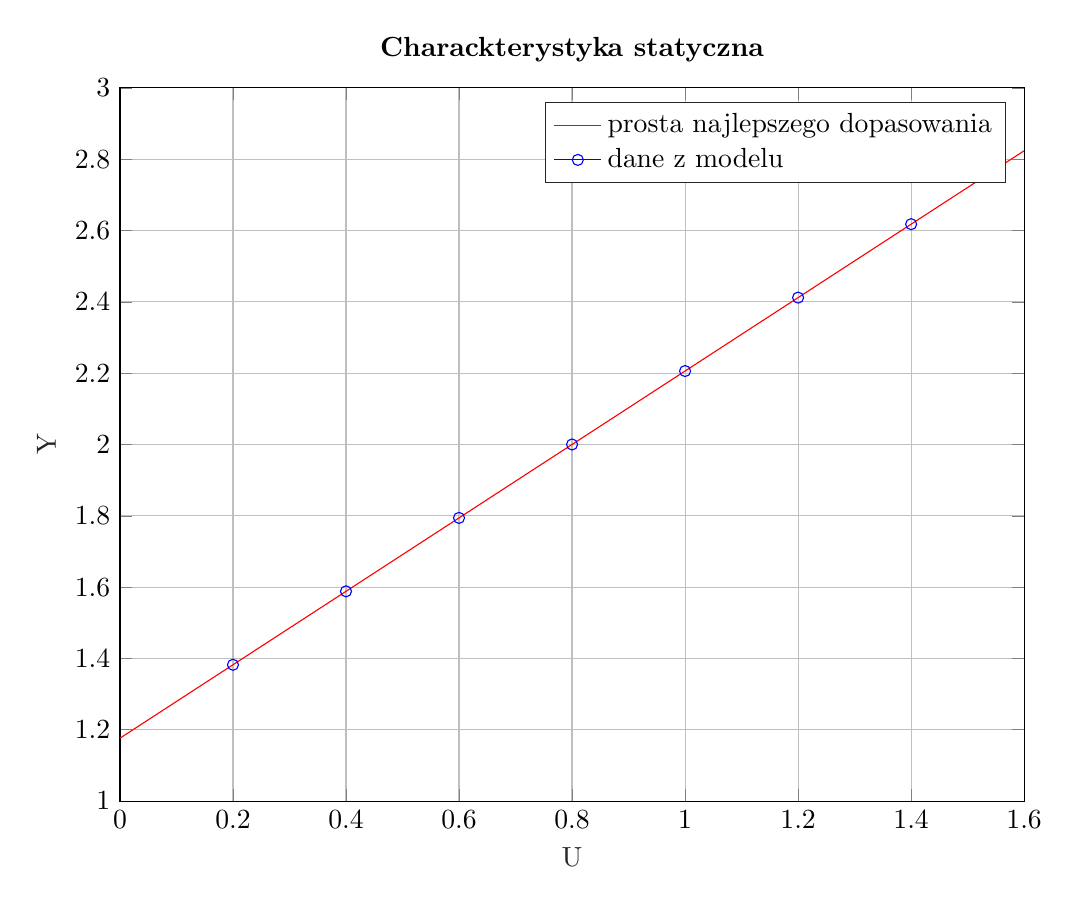
\begin{tikzpicture}

\begin{axis}[%
width=4.521in,
height=3.566in,
at={(0.758in,0.481in)},
scale only axis,
xmin=0,
xmax=1.6,
xlabel style={font=\color{white!15!black}},
xlabel={U},
ymin=1,
ymax=3,
ylabel style={font=\color{white!15!black}},
ylabel={Y},
axis background/.style={fill=white},
title style={font=\bfseries},
title={Charackterystyka statyczna},
xmajorgrids,
ymajorgrids,
legend style={legend cell align=left, align=left, draw=white!15!black}
]
\addplot [color=red]
  table[row sep=crcr]{%
0	1.17631908206646\\
0.1	1.27927919680815\\
0.2	1.38223931154984\\
0.3	1.48519942629154\\
0.4	1.58815954103323\\
0.5	1.69111965577492\\
0.6	1.79407977051661\\
0.7	1.89703988525831\\
0.8	2\\
0.9	2.10296011474169\\
1	2.20592022948338\\
1.1	2.30888034422508\\
1.2	2.41184045896677\\
1.3	2.51480057370846\\
1.4	2.61776068845015\\
1.5	2.72072080319185\\
1.6	2.82368091793354\\
};
\addlegendentry{prosta najlepszego dopasowania}

\addplot [color=blue, draw=none, mark=o, mark options={solid, blue}]
  table[row sep=crcr]{%
0.2	1.38223931154985\\
0.4	1.58815954103323\\
0.6	1.79407977051661\\
0.8	2\\
1	2.20592022948339\\
1.2	2.41184045896677\\
1.4	2.61776068845015\\
};
\addlegendentry{dane z modelu}

\end{axis}
\end{tikzpicture}%
\end{figure}

Aby otrzymać odpowiedź skokową wykorzystywaną w algorytmie DMC należy pobudzić obiekt skokiem jednostkowym, gdzie od chwili zerowej sygnał sterujący ma wartość 1, a w przeszłości jest zerowy. Wynik tej odpowiedzi skokowej jest przedstawiony na rys //TODO
\begin{figure}
	//TODO
\end{figure}
<<<<<<< HEAD
<<<<<<< HEAD
<<<<<<< HEAD
<<<<<<< HEAD

\section{Programy do symulacji algorytmów}
Programy do symulacji algorytmów zostały zaimplementowane w plikach \texttt{PID.m} i \texttt{DMC.m}. Funkcje te są wywoływane w każdej kolejnej dyskretnej chwili $k$ i obliczają wartość sterowania jaką należy przesłać na obiekt. Na wejście przyjmują więc obecne wartości zmiennych (PID - uchyb $E$, numer dyskretnej chwili $k$, parametry regulatora dyskretnego $r_{\mathrm{0}}$, $r_{\mathrm{1}}$, $r_{\mathrm{2}}$ i wartość punktu pracy $U_{\mathrm{pp}}$, a DMC dodatkowo jeszcze macierze $K$, $M_{\mathrm{P}}$, wektor $\Delta U_{\mathrm{P}}$). Nakładają one także omówione wcześniej ograniczenia na sygnał sterujący. Funkcje te wywoływane są przez funkcje przeprowadzające symulacje \texttt{PIDsimulation.m} i \texttt{DMCsimulation.m}, które to z kolei zwracają wartości wyjścia, sterowania i wskaznika jakości i przekazują je do głównego programu.

\section{Ręczny dobór odpowiednich wartości parametrów}
Nastawy regulatora PID i parametry regulatora DMC dobieraliśmy metodą eksperymentalną, tj powoli i cierpliwie zmieniając ich wartości oraz obserwując rysunki przedstawiające przebiegi wyjścia procesu. Jak się okazuje optymalnie działający regulator PID przy nastawach ręcznych otrzymaliśmy przy następujących wartościach: $K=\num{0.01}$, $T_\mathrm{i}=10000$, $T_\mathrm{d}=0$, natomiast wskaznik jakości przyjął w tym wypadku wartość $E=\num{122.243}$. Dla algorytmu DMC optymalnymi okazały się parametry: $N=200$, $N_\mathrm{u}=15$, $\lambda=1$. Wyniki symulacji z takimi parametrami znajdują się na rysunkach: //TODO
\section{Optymalizacja wskaźnika jakości}
=======
=======
>>>>>>> 1aa569faa9f60a46403ca971df9c995fe9adabf0
=======
>>>>>>> 1aa569faa9f60a46403ca971df9c995fe9adabf0
=======
>>>>>>> 1aa569faa9f60a46403ca971df9c995fe9adabf0

\section{Programy do symulacji algorytmów}
Programy do symulacji algorytmów zostały zaimplementowane w plikach \texttt{PID.m} i \texttt{DMC.m}. Funkcje te są wywoływane w każdej kolejnej dyskretnej chwili $k$ i obliczają wartość sterowania jaką należy przesłać na obiekt. Na wejście przyjmują więc obecne wartości zmiennych (PID - uchyb $E$, numer dyskretnej chwili $k$, parametry regulatora dyskretnego $r_{\mathrm{0}}$, $r_{\mathrm{1}}$, $r_{\mathrm{2}}$ i wartość punktu pracy $U_{\mathrm{pp}}$, a DMC dodatkowo jeszcze macierze $K$, $M_{\mathrm{P}}$, wektor $\Delta U_{\mathrm{P}}$). Nakładają one także omówione wcześniej ograniczenia na sygnał sterujący. Funkcje te wywoływane są przez funkcje przeprowadzające symulacje \texttt{PID\_simulation.m} i \texttt{DMC\_simulation.m}, które to z kolei zwracają wartości wyjścia, sterowania i wskaznika jakości i przekazują je do głównego programu.

\section{Ręczny dobór odpowiednich wartości parametrów}
Nastawy regulatora PID i parametry regulatora DMC dobierano metodą eksperymentalną, tj powoli i cierpliwie zmieniając ich wartości oraz obserwując rysunki przedstawiające przebiegi wyjścia procesu. Jak się okazuje optymalnie działający regulator PID przy nastawach ręcznych otrzymaliśmy przy następujących wartościach: $K=\num{0.01}$, $T_\mathrm{i}=10000$, $T_\mathrm{d}=0$, natomiast wskaznik jakości przyjął w tym wypadku wartość $E=\num{122.243}$. Dla algorytmu DMC jakościowo dobre okazały się parametry: $N=50$, $N_\mathrm{u}=1$, $\lambda=\num{1.5}$. Wskaźnik jakości dla tych paramterów przyjął wartość $E=\num{60.614}$  Wyniki symulacji z takimi parametrami znajdują się na rysunkach: //TODO
\section{Optymalizacja wskaźnika jakości}
Następnie dokonano optymalizacji wskaźnika jakości regulatorów PID i DMC dla tej samej trajektorii z wykorzystaniem funkcji wbudowanych w środowisku Matlab. Za przyjęty wskaźnik jakości przyjęto sumę kwadratrów róznic pomiędzy wartością zadaną, a wartością wyjścia symulowanego obiektu:

\begin{equation}
E = \sum_{k=1}^{N} (Y^{zad}(k)-Y(k))^2
\end{equation}

Dla regulatora PID do doboru optymalnych parametrów wykorzystano funkcję 
\verb+fmincon+. //TODO: PID do opisania

<<<<<<< HEAD
<<<<<<< HEAD
<<<<<<< HEAD
W przypadku regulatora DMC ze względu na parametry $N$, $N_u$ przyjmujące wartości całkowite należało zastosować funkcję umożliwiającą optymalizację wskaźnika jakości dla parametrów o wartościach całkowitych. W tym celu wykorzystano funkcję \verb+ga+, czyli funkcję wykorzystującą algorytm genetyczny do optymalizacji. W ten sposób otrzymano parametry $N=43$, $N_\mathrm{u}=1$, $\lambda=\num{1.0555}$. Wskaźnik jakości dla tych parametrów wynosi $E=\num{60.369}$.
>>>>>>> 1aa569faa9f60a46403ca971df9c995fe9adabf0
=======
W przypadku regulatora DMC ze względu na parametry $N$, $N_u$ przyjmujące wartości całkowite należało zastosować funkcję umożliwiającą optymalizację wskaźnika jakości dla parametrów o wartościach całkowitych. W tym celu wykorzystano funkcję \verb+ga+, czyli funkcję wykorzystującą algorytm genetyczny do optymalizacji. W ten sposób otrzymano parametry $N=43$, $N_\mathrm{u}=1$, $\lambda=\num{1.0555}$. Wskaźnik jakości dla tych parametrów wynosi $E=\num{60.369}$.
>>>>>>> 1aa569faa9f60a46403ca971df9c995fe9adabf0
=======
W przypadku regulatora DMC ze względu na parametry $N$, $N_u$ przyjmujące wartości całkowite należało zastosować funkcję umożliwiającą optymalizację wskaźnika jakości dla parametrów o wartościach całkowitych. W tym celu wykorzystano funkcję \verb+ga+, czyli funkcję wykorzystującą algorytm genetyczny do optymalizacji. W ten sposób otrzymano parametry $N=43$, $N_\mathrm{u}=1$, $\lambda=\num{1.0555}$. Wskaźnik jakości dla tych parametrów wynosi $E=\num{60.369}$.
>>>>>>> 1aa569faa9f60a46403ca971df9c995fe9adabf0
=======
W przypadku regulatora DMC ze względu na parametry $N$, $N_u$ przyjmujące wartości całkowite należało zastosować funkcję umożliwiającą optymalizację wskaźnika jakości dla parametrów o wartościach całkowitych. W tym celu wykorzystano funkcję \verb+ga+, czyli funkcję wykorzystującą algorytm genetyczny do optymalizacji. W ten sposób otrzymano parametry $N=43$, $N_\mathrm{u}=1$, $\lambda=\num{1.0555}$. Wskaźnik jakości dla tych parametrów wynosi $E=\num{60.369}$.
>>>>>>> 1aa569faa9f60a46403ca971df9c995fe9adabf0
